\documentclass[a4paper,11pt]{article}
\usepackage{amsmath,amsthm,amsfonts,amssymb,amscd,amstext,vmargin,graphics,graphicx,tabularx,multicol} \usepackage[french]{babel}
\usepackage[utf8]{inputenc}  
\usepackage[T1]{fontenc} 
\usepackage[T1]{fontenc}
\usepackage{amsmath,amssymb}
\usepackage{pstricks-add,tikz,tkz-tab,variations}
\usepackage[autolanguage,np]{numprint} 
\usepackage{color}
\usepackage{ulem}
\usepackage{pifont}


\setmarginsrb{1.5cm}{0.5cm}{1cm}{0.5cm}{0cm}{0cm}{0cm}{0cm} %Gauche, haut, droite, haut
\newcounter{numexo}
\newcommand{\exo}[1]{\stepcounter{numexo}\noindent{\bf Exercice~\thenumexo} : \marginpar{\hfill /#1}}
\reversemarginpar


\newcounter{enumtabi}
\newcounter{enumtaba}
\newcommand{\q}{\stepcounter{enumtabi} \theenumtabi.  }
\newcommand{\qa}{\stepcounter{enumtaba} (\alph{enumtaba}) }
\newcommand{\initq}{\setcounter{enumtabi}{0}}
\newcommand{\initqa}{\setcounter{enumtaba}{0}}

\newcommand{\be}{\begin{enumerate}}
\newcommand{\ee}{\end{enumerate}}
\newcommand{\bi}{\begin{itemize}}
\newcommand{\ei}{\end{itemize}}
\newcommand{\bp}{\begin{pspicture*}}
\newcommand{\ep}{\end{pspicture*}}
\newcommand{\bt}{\begin{tabular}}
\newcommand{\et}{\end{tabular}}
\renewcommand{\tabularxcolumn}[1]{>{\centering}m{#1}} %(colonne m{} centrée, au lieu de p par défault) 
\newcommand{\tnl}{\tabularnewline}

\newcommand{\trait}{\noindent \rule{\linewidth}{0.2mm}}
\newcommand{\hs}[1]{\hspace{#1}}
\newcommand{\vs}[1]{\vspace{#1}}

\newcommand{\N}{\mathbb{N}}
\newcommand{\Z}{\mathbb{Z}}
\newcommand{\R}{\mathbb{R}}
\newcommand{\C}{\mathbb{C}}
\newcommand{\Dcal}{\mathcal{D}}
\newcommand{\Ccal}{\mathcal{C}}
\newcommand{\mc}{\mathcal}

\newcommand{\vect}[1]{\overrightarrow{#1}}
\newcommand{\ds}{\displaystyle}
\newcommand{\eq}{\quad \Leftrightarrow \quad}
\newcommand{\vecti}{\vec{\imath}}
\newcommand{\vectj}{\vec{\jmath}}
\newcommand{\Oij}{(O;\vec{\imath}, \vec{\jmath})}
\newcommand{\OIJ}{(O;I,J)}

\newcommand{\textding}[1]{\text{\ding{#1}}}

\newcommand{\bmul}[1]{\begin{multicols}{#1}}
\newcommand{\emul}{\end{multicols}}


\newcommand{\reponse}[1][1]{%
\multido{}{#1}{\makebox[\linewidth]{\rule[0pt]{0pt}{20pt}\dotfill}
}}

\newcommand{\titre}[5] 
% #1: titre #2: haut gauche #3: bas gauche #4: haut droite #5: bas droite
{
\noindent #2 \hfill #4 \\
#3 \hfill #5

\vspace{-1.6cm}

\begin{center}\rule{6cm}{0.5mm}\end{center}
\vspace{0.2cm}
\begin{center}{\large{\textbf{#1}}}\end{center}
\begin{center}\rule{6cm}{0.5mm}\end{center}
}



\begin{document}
\pagestyle{empty}
\titre{Devoir maison - Les transformations pas à pas}{Nom}{Prénom}{Date}{Classe}


\section{\underline{La symétrie axiale}}

\bmul{2}


\textding{48}  \textbf{MÉTHODE AVEC DES CARREAUX}\\
 
\includegraphics[scale=1]{axiale.eps} \\

\columnbreak

\textbf{\underline{Exercice d'application 1 :}} A vous de jouer! Tracer les symétriques des figures suivantes par rapport à la droite (d).\\

\includegraphics[scale=0.55]{axiale3.eps} \\

\emul


 \textding{48} \textbf{MÉTHODE SUR FEUILLE BLANCHE}\\
\includegraphics[scale=0.9]{axiale2.eps} \\

\textbf{\underline{Exercice d'application 2 :}} A vous de jouer ! Tracer le symétrique de la figure ci-dessous par rapport à la droite.
\begin{center}
\includegraphics[scale=1]{axiale4.eps} 
\end{center}



\newpage


\section{\underline{La symétrie centrale}}

\bmul{2}

 \textding{48} \textbf{MÉTHODE AVEC DES CARREAUX}\\
 
 Ci-dessous, on a construit le point A' symétrique du point A par rapport au point O.\\
\includegraphics[scale=1]{centrale1.eps} \\


\columnbreak

\textbf{\underline{Exercice d'application 3 :}}\\
A vous de jouer ! Tracer le symétrique de la figure ci-dessous par rapport au point R.
\begin{center}
\includegraphics[scale=0.7]{centrale3.eps} 
\end{center}

\emul


\bmul{2}

 \textding{48} \textbf{MÉTHODE SUR FEUILLE BLANCHE}\\
  Ci-dessous, on a construit le point A' symétrique du point A par rapport au point O.\\
\includegraphics[scale=0.9]{centrale2.eps} 


\columnbreak

\textbf{\underline{Exercice d'application 4 :}}\\
A vous de jouer ! Tracer le symétrique de la figure ci-dessous par rapport au point A.\\
\begin{flushleft}
\includegraphics[scale=0.5]{centrale4.eps} 
\end{flushleft}


\emul
\section{\underline{La translation}}

\bmul{2}

 \textding{48} \textbf{MÉTHODE AVEC DES CARREAUX}\\
 
   Ci-dessous, on a construit l'image du triangle ABC par la translation qui transforme D en E.\\
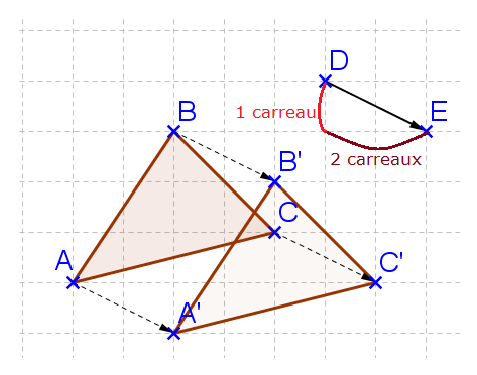
\includegraphics[scale=1.1]{translation3.eps} \\



\columnbreak

\textbf{\underline{Exercice d'application 5 :}}\\
A vous de jouer ! Construire l'image de la figure ci-dessous par la translation qui transforme B en C.\\

\includegraphics[scale=0.85]{translation1.eps} \\

\emul

\newpage


 \textding{48} \textbf{MÉTHODE SUR FEUILLE BLANCHE}\\
\includegraphics[scale=0.9]{translation4.eps} \\

\textbf{\underline{Exercice d'application 6 :}}\\
A vous de jouer ! Construire l'image de la figure ci-dessous par la translation qui transforme D en D'.\\
\includegraphics[scale=0.69]{translation2.eps} 





\section{\underline{La rotation}}


 \textding{48} \textbf{MÉTHODE SUR FEUILLE BLANCHE}\\
 
Ci-dessous, on a construit l'image du point M par la rotation de centre P et d'angle 70\degre dans le anti-horaire.
\begin{flushleft}
\includegraphics[scale=0.85]{rotation1.eps} 
\end{flushleft}

\newpage

\textbf{\underline{Exercice d'application 7 :}}\\
Construire l'image du triangle rectangle AGH par la rotation de centre I et d'angle 90\degre dans le sens anti-horaire.\\
\includegraphics[scale=0.9]{rotation2.eps} \\

\textbf{\underline{Exercice d'application 8:}}\\
Construire l'image de la figure ci-dessous par la rotation de centre O et d'angle 90\degre dans le sens anti-horaire.\\
\begin{center}
\includegraphics[scale=0.9]{rotation3.eps} \\
\end{center}


\textbf{\underline{Exercice d'application 9 :}} BILAN\\
\bmul{2}
\begin{flushleft}
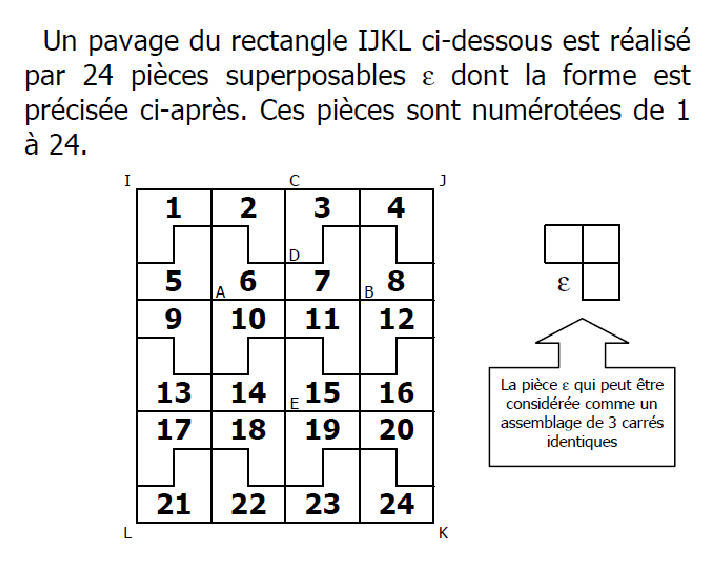
\includegraphics[scale=0.75]{rotation4.eps} 
\end{flushleft}

\columnbreak

Compléter les phrases suivantes, sans justification :\\

a)La symétrie d'axe (CE) transforme la pièce 17 en
la pièce . . .\\

b) La symétrie de centre B transforme la pièce 3 en
la pièce . . .\\

c) La translation de vecteur CB transforme la pièce
3 en la pièce . . .\\

d) La rotation de centre E et d'angle 90\degre, dans le
sens des aiguilles d'une montre, transforme la pièce
15 en la pièce . . .\\

\emul


\end{document}
